\subsection{Simulation of the Filter}
The position Kalman filter is also tuned and tested utilizing simulations. These are performed by applying some inputs to the simulation model of the system. The signals coming out of the model are then extracted and some noise is added to them. The noisy signals are used as the input to the position Kalman filter in order to evaluate its performance. The amount of noise added is the same as that present in the real sensors, whose variances are seen in \autoref{app:IMUVariances}.

As in the case of the attitude, the tuning is done by choosing the appropriate values for the covariance matrix of the states, $\vec{Q}_\mathrm{pos}$. 

This procedure starts by obtaining a good estimation of the accelerations in the body frame, $\ddot{x}_\mathrm{b}$ and $\ddot{y}_\mathrm{b}$, since the other estimations depend on these. The result can be seen in \autoref{fig:sim_xbddot}, where the measurement, the estimation and the real value of $\ddot{x}_\mathrm{b}$ are depicted.
\begin{figure}[H]
    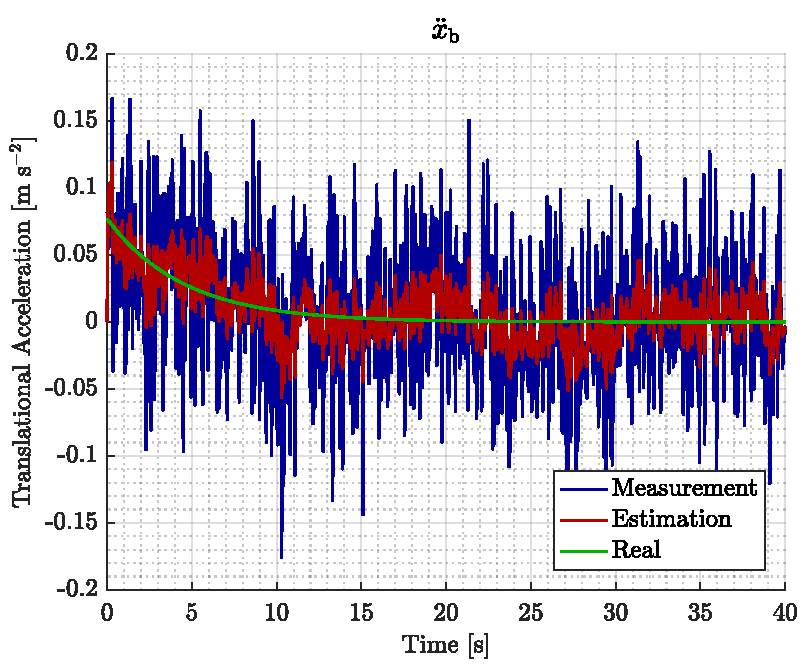
\includegraphics[width=0.5\textwidth]{figures/sim_xbddot}
    \caption{ Measurement, real value and estimation of $\ddot{x}_\mathrm{b}$}
    \label{fig:sim_xbddot}
\end{figure}
It is noticeable that the filter reduces most of the noise present on the measurement and gives a good estimation of the acceleration in the body frame.
 
Then, the velocities, $\dot{x}_\mathrm{b}$ and $\dot{y}_\mathrm{b}$ estimations are tuned. These do not rely on any measurements and are mainly the result of integrating the acceleration as seen in the model used for the position Kalman filter, see \autoref{eq:Apos}. The result for these signal is seen in \autoref{fig:sim_xbdot}, where
\begin{figure}[H]
	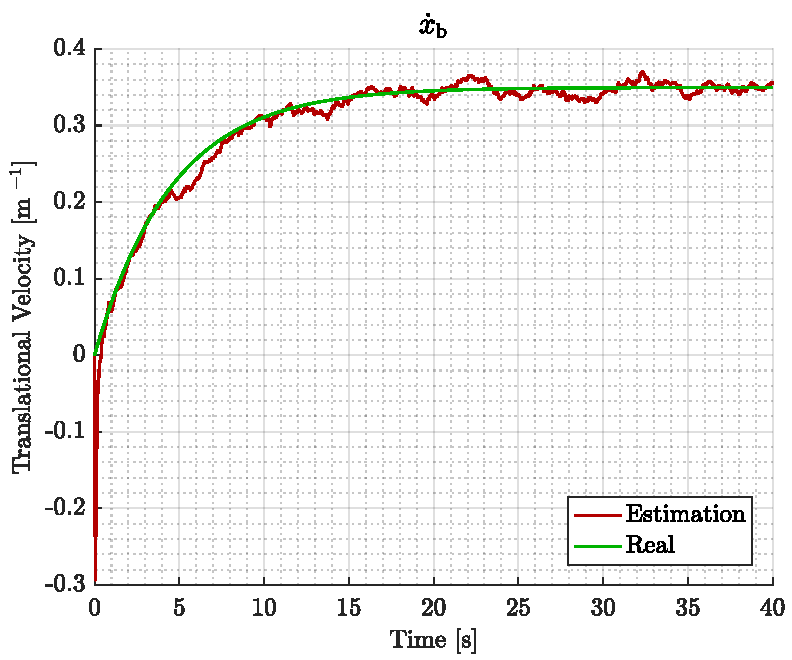
\includegraphics[width=0.5\textwidth]{figures/sim_xbdot}
	\caption{ Real value and estimation of $\dot{x}_\mathrm{b}$}
	\label{fig:sim_xbdot}
\end{figure}
The estimation of $\dot{x}_\mathrm{b}$ gives a good result even though there is no direct measurement of the velocity.

Finally, the estimation of the positions in the NED frame, $x_\mathrm{n}$ and $y_\mathrm{n}$, are tuned, these depend on the accelerations and velocities estimations and on the position measurements coming from the RTK GPS module. \autoref{fig:sim_xn} shows the result in an X-Y plot of the position of the vessel.
\begin{figure}[H]
	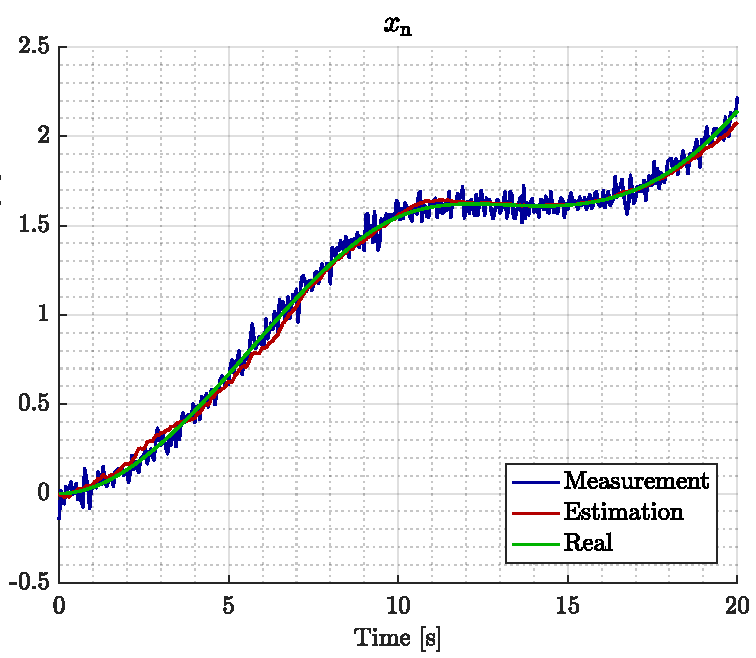
\includegraphics[width=0.5\textwidth]{figures/sim_xn}
	\caption{ Measurement, real value and estimation of the X-Y position of the vessel in the NED frame.}
	\label{fig:sim_xn}
\end{figure}      
As it can be observed, the estimation approximates well the real value and the Kalman filter removes most of the noise added by the GPS.

The final covariance matrix for the states obtained after the tuning process is
% 
\begin{flalign}
    \vec{Q}_\mathrm{pos} &= \mathrm{diag}\left(0,0,0,0,0,0,0,0,0 \right)\ .
\end{flalign}
